\chapter{Biorthogonalization Methods}

Not all Krylov subspace iterations for nonsymmetric systems involve recurrences of growing length and growing cost. Methods based on three-term recurrences have also been devised, and they are the most powerful nonsymmetric iterations available today. The price to be paid, at least for some of the iterations in this category, is that one must work with two Krylov subspaces rather than one, generated by multiplications by $A^*$ as well as $A$.  

\section{Where We Stand} 
We have shown a table of Krylov subspace matrix iterations: 
%────────────────────────────────────────
\begin{figure}[H]
    \centering
    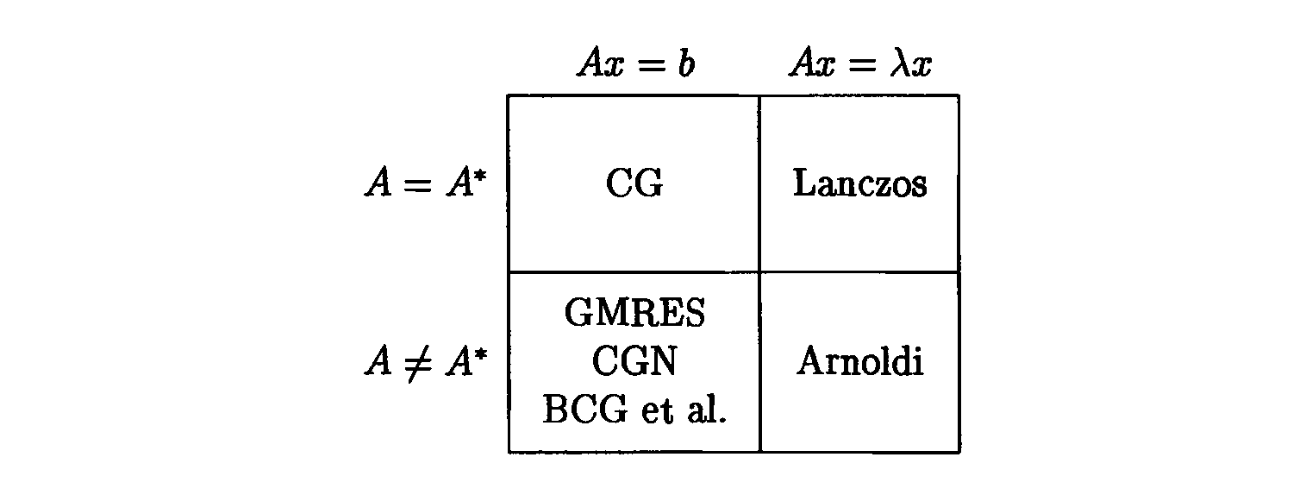
\includegraphics[width=0.8\textwidth]{figures/39-1.png}
\end{figure}
%────────────────────────────────────────
Our discussions of three of these boxes are now complete, and as for the fourth, lower-left position, we have already discussed GMRES. In this lecture we turn to the final two lines of the table. We spend just a moment on CGN, a simple and easily analyzed algorithm, and then move to our main subject, the biorthogonalization methods represented by the entry ``BCG et al.'' 

\section{CGN = CG Applied to the Normal Equations} 
Let $ A \in \CC^{ m\times m }  $ be nonsingular but not hermitian, and we want to solve $ Ax=b $. One of the simplest methods is to apply the CG iteration to the normal equations: 
\begin{equation}
\label{eq: CGN normal equations}
    A^* A x = A^* b.    
\end{equation}

(The matrix $A^* A$ is not formed explicitly, which would require $m^3$ flops. Instead, each matrix-vector product $A^* A v$ is evaluated in two steps as $A^*(A v)$.) Now we can apply the CG method. This method goes by the name of CGN (also CGNR), which roughly stands for ``CG applied to the normal equations.''

Similarly, from Thm~\ref{thm: Properties of CG}, we have 
\[
    x_n \in \langle A^* b, (A^* A)A^* b, \ldots , (A^* A)^{n-1}A^* b \rangle .
\]

From Thm~\ref{thm: Optimality of CG}, we know that the $ A^* A $-norm of the error is minimized over this space at each step, and since $ \|e_n\|_{A^* A}^{2}  = e_n^* A^* A e_n = \|Ae_n\|_2^{2}  = \|r_n\|^{2} , $ this is another way of saying that the 2-norm of the residual $ r_n=b-Ax_n $ is minimized. Thus CGN, like GMRES, is a minimal residual method, but since their Krylov subspaces are different, these tw methods are by no means equivalent.  

According to Theorem~\ref{thm: Convergence of CG} the convergence of CGN is controlled by the eigenvalues of $A^* A$. These numbers are equal to the squares of the singular values of $A$. Thus the convergence of CGN is determined by the singular values of $A$, and in principle has nothing to do with the eigenvalues of $A$. The fact that squares are involved is unfortunate, however. If $A$ has condition number $\kappa$, then $A^* A$ has condition number $\kappa^2$, and the rate for CGN becomes
$$
\frac{\left\|r_n\right\|_2}{\left\|r_0\right\|_2} \leq 2\left(\frac{\kappa-1}{\kappa+1}\right)^n.
$$
For large $\kappa$, this is much more worse; it implies that $O(\kappa)$ iterations are required for convergence to a fixed accuracy, not $O(\sqrt{\kappa})$. 

This "squaring of the condition number" has given the CGN iteration a poor reputation, which, on balance, may be deserved. Nevertheless, for some problems CGN vastly outperforms alternative methods, since their convergence depends on eigenvalues rather than singular values. All one needs is a matrix whose singular values are well behaved but whose eigenvalues are not, such as a well-conditioned matrix whose spectrum surrounds the origin in the complex plane. An extreme example is provided by the $m \times m$ circulant matrix of the form

\[
    A = \begin{bmatrix}[] 
        0 & 1 &  &  &   \\
         & 0 & 1 &  &   \\
         &  & 0 & 1 &   \\
         &  &  & 0 &  1 \\
        1 &  &  &  &  0 \\
    \end{bmatrix}. 
\]
The singular values of this matrix are all equal to $ 1 $, but the eigenvalues are the $ m $th roots of unity. GMRES requires $ m $ steps for convergence for a general right-hand side $ b $, while CGN converges in one step. 

Another virtue of the CGN iteration is that since it is based on the normal equations, it applies without modification to least squares problems, while $ A $ is no longer square.

\section{Tridiagonal Biorthogonalization}
The Lanczos iteration is a process of tridiagonal orthogonalization. It $ A $ is not hermitian, such a reduction is not possible in general. The Arnoldi iteration, a process of Hessenberg orthogonalization, doe the latter. 

Biorthogonalization methods are based on the opposite choice. If we insist on a tridiagonal result but give up the use of unitary transformations, we have a process of \textbf{tridiagonal biorthogonalization}: $ A = VTV^{-1}  $, where $ V $ is nonsingular but not unitary. 

To begin to make this idea into an iterative algorithm, we must see what is involved for $ n<m $. Assume $ V $ is nonsingular and $ A = VTV^{-1}  $ with $ T $ tridiagonal, and let $ W= V^{-*} $. Let $ v_j $ and $ w_j $ denote the $ j$th columns of $ V $ and $ W $, respectively. We can see that 
\[
    W^* V = I \Rightarrow w_i^* v_j  = \delta _{ij}.    
\]
Now we define $ V_n = (v_1,\ldots ,v_n) , W_n = (w_1,\ldots ,w_n) \in \RR^{m\times n} $. Then, 
\[
    W_n^* V_n = V_n^* W_n = I_n. 
\]
Recall that for the Lanczos iterations, we have 
\[
    AQ_n = Q_{n+1}\tilde T_n, \quad T_n = Q_n^*  A Q_n. 
\]
For the Arnoldi iteration,  we have 
\[
    AQ_n = Q_{n+1}\tilde H_n, \quad H_n = Q_n^* A Q_n.
\]
Then for the biorthogonalization methods, we have 
\begin{align}
    AV_n = V_{n+1}\tilde T_n, \label{eq: bi AVT}\\ 
    A^* W_n = W_{n+1}\tilde S_n , \label{eq: bi AWS} \\ 
    T_n = S_n^*  = W_n^* A V_n. \label{eq: bi TSAW} 
\end{align}
Note that here $ \tilde T_{n+1} $ and $ \tilde S_{n+1}$ are tridiagonal matrices with dimension $ (n+1)\times n $, and $ T_n = S_n^*  $ is the $ n\times n $ matrix obtained by deleting the last row of $ \tilde T_{n+1} $ or the last column of $ \tilde S_{n+1}^*  $. NOte that \eqref{eq: bi AVT} can displayed as 
\[
A (v_1,\ldots ,v_n) = (v_1, v_2,\ldots ,v_{n+1})\begin{bmatrix}[] 
    \alpha _1 & \gamma _1 &  &  &   \\
    \beta _1 & \alpha _2 & \gamma _2 &  &   \\
     & \beta _2 & \alpha _3 & \ddots &   \\
     &  & \ddots & \ddots &  \gamma _{n-1} \\
     &  &  & \beta _{n-1} &  \alpha _n \\
     &  &  &  &  \beta _n \\
\end{bmatrix} ,
\]

which corresponds to the three-term recurrence relation 
\begin{equation}
\label{eq: BiCG three-term}
    Av_n = \gamma _{n-1}v_{n-1} + \alpha _n v_n + \beta _n v_{n+1}. 
\end{equation}

Similarly, \eqref{eq: bi AWS} takes the form 
\[
    A^* (w_1,\ldots ,w_n) = (w_1,\ldots ,w_{n+1}) \begin{bmatrix}[] 
        \bar \alpha _1 & \bar \beta _1 &  &  &   \\
        \bar \gamma _1 & \bar \alpha _2 & \bar \beta _2 &  &   \\
         & \bar \gamma_2 & \bar \alpha _3 & \ddots &   \\
         &  & \ddots & \ddots &  \bar \beta _{n-1} \\
         &  &  & \bar \gamma _{n-1}  &  \bar \alpha _n \\
         &  &  &  &  \bar \gamma _n \\
    \end{bmatrix}, 
\]
corresponding to 
\begin{equation}
\label{eq: BICG three-term aw}
    A^* w_n = \bar \beta _{n-1} w_{n-1} + \bar \alpha _n w_n + \bar \gamma _n w_{n+1}. 
\end{equation}

As usual with Krylov subspace iterations, these equations suggest an algorithm. Begin with vectors $v_1$ and $w_1$ that are arbitrary except for satisfying $v_1^* w_1=1$, and set $\beta_0=\gamma_0=0$ and $v_0=w_0=0$. Now, for each $n=1,2, \ldots$, set $\alpha_n=w_n^* A v_n$, as follows from \eqref{eq: bi TSAW}. The vectors $v_{n+1}$ and $w_{n+1}$ are then determined by \eqref{eq: BiCG three-term} and \eqref{eq: BICG three-term aw} up to scalar factors. These factors may be chosen arbitrarily, subject to the normalization $w_{n+1}^* v_{n+1}=1$, whereupon $\beta_{n+1}$ and $\gamma_{n+1}$ are determined by \eqref{eq: BiCG three-term} and \eqref{eq: BICG three-term aw}.  

For a generic matrix, in exact arithmetic, the procedure will run to completion after $m$ steps, but for certain special matrices there may also be a breakdown of the process before this point. If $v_n=0$ or $w_n=0$ at some step, an invariant subspace of $A$ or $A^*$ has been found: the tridiagonal matrix $T$ is reducible. Alternatively, it may also happen that $v_n \neq 0$ and $w_n \neq 0$ but $w_n^* v_n=0$. The possibility of this more serious kind of breakdown is present in most biorthogonalization methods. As in other areas of numerical analysis, the fact that exact breakdown is possible for certain problems implies that near-breakdown may occur for many other problems, with potentially adverse consequences in floating point arithmetic. Some methods for coping with these phenomena are mentioned at the end of this lecture.

\section{BCG=Biconjugate Gradients}

One way to use the biorthogonalization process just described is to compute eigenvalues: as $n \rightarrow \infty$, some eigenvalues of $T_n$ may converge rapidly to some eigenvalues of $A$. Another application, which we shall now briefly discuss, is the solution of nonsingular systems of equations $A x=b$. The classic algorithm of this type is known as biconjugate gradients or $B C G$.

The principle of BCG is as follows. We take $v_1=b$, so that the first Krylov subspace becomes $\mathcal{K}_n=\left\langle b, A b, \ldots, A^{n-1} b\right\rangle$. Recall that the principle of GMRES is to pick $x_n \in \mathcal{K}_n$ so that the orthogonality condition
GMRES: $\quad r_n \perp\left\langle A b, A^2 b, \ldots, A^n b\right\rangle=A \mathcal{K}_n$
is satisfied, where $r_n=b-A x_n$ is the residual corresponding to $x_n$. This choice has the effect of minimizing $\left\|r_n\right\|$, the 2-norm of the residual. The principle of the BCG algorithm is to pick $x_n$ in the same subspace, $x_n \in \mathcal{K}_n$, but to enforce the orthogonality condition
GMRES: $\quad r_n \perp\left\langle A b, A^2 b, \ldots, A^n b\right\rangle=A \mathcal{K}_n$
is satisfied, where $r_n=b-A x_n$ is the residual corresponding to $x_n$. This choice has the effect of minimizing $\left\|r_n\right\|$, the 2 -norm of the residual. The principle of the BCG algorithm is to pick $x_n$ in the same subspace, $x_n \in \mathcal{K}_n$, but to enforce the orthogonality condition
$$
\text { BCG: } \quad r_n \perp\left\langle w_1, A^* w_1, \ldots,\left(A^*\right)^{n-1} w_1\right\rangle .
$$
Here $w_1 \in \mathbb{C}^m$ is an arbitrary vector satisfying $w_1^* v_1=1$; in applications one sometimes takes $w_1=v_1 /\left\|v_1\right\|_2$. Unlike GMRES, this choice does not minimize $\left\|r_n\right\|_2$, and it is not optimal from the point of view of minimizing the number of iterations. Its advantage is that it can be implemented with three-term recurrences rather than the $(n+1)$-term recurrences of GMRES.

Without giving details of the derivation, we now record the BCG algorithm in its standard form. What follows should be compared with Algorithm 38.1, the CG algorithm. The two are the same except that the sequence of search directions $\left\{p_n\right\}$ of CG has become two sequences $\left\{p_n\right\}$ and $\left\{q_n\right\}$, and the sequence of residuals $\left\{r_n\right\}$ of CG has become two sequences $\left\{r_n\right\}$ and $\left\{s_n\right\}$.


\begin{algorithm}[H]
    \caption{Biconjugate Gradient (BCG) iteration}
    \label{Algo 39.1}
    $ x_0=0, p_0=r_0=b, q_0=s_0=\text { arbitrary } $\; 
    \For{$ n=1,2,3,\ldots  $}{ 
        $ \alpha _n = s_{n-1}^*  r_{n-1}) / (q_{n-1}^*  A p_{n-1}) $\; 
        $ x_n = x_{n-1} +\alpha _n p_{n-1} $\; 
        $ r_n = r_{n-1} - \alpha _n A p_{n-1} $\; 
        $ s_n = s_{n-1} -\alpha _n A^* q_{n-1} $\; 
        $ \beta _n = (s_n^* r_n) /( s_{n-1}^* r_{n-1}) $\;
        $ p_n = r_n + \beta _n p_{n-1} $\; 
        $ q_n = s_n + \beta _n q_{n-1} $\;
     } 
\end{algorithm}

\section{Example} 
We consider the same example in chapter 37 except with one change: the sign of all the entries are randomized. This makes the matrix no longer hermitian, and it changes the dominat entries on the diagonal to $ 1 $ and $ -1 $ at random, rather than all $1 $. Now the eigenvalues are clustered around $ 1 $ and $ -1 $ instead of just $ 1 $. 

In this figure we set $ \tau = 0.01 $. with $\tau=0.01$. Considering first the GMRES curve, we note that the convergence is half as fast as in Chapter 37, with essentially no progress at each odd-numbered step, but steady progress at each even step. This odd-even effect is a result of the approximate $\pm 1$ symmetry of the matrix: a polynomial $p(z)$ of degree $2 k+1$ with $p(0)=1$ can be no smaller at 1 and -1 than a corresponding polynomial of degree $2 k$. Turning now to the BCG curve, we see that the convergence is comparable in an overall sense, but it is no longer monotonic, showing spikes of magnitude as great as about $10^2$ at each oddnumbered step. The accuracy attained at the end has also suffered by more than a digit. All of these features are typical of BCG computations.
%────────────────────────────────────────
\begin{figure}[H]
    \centering
    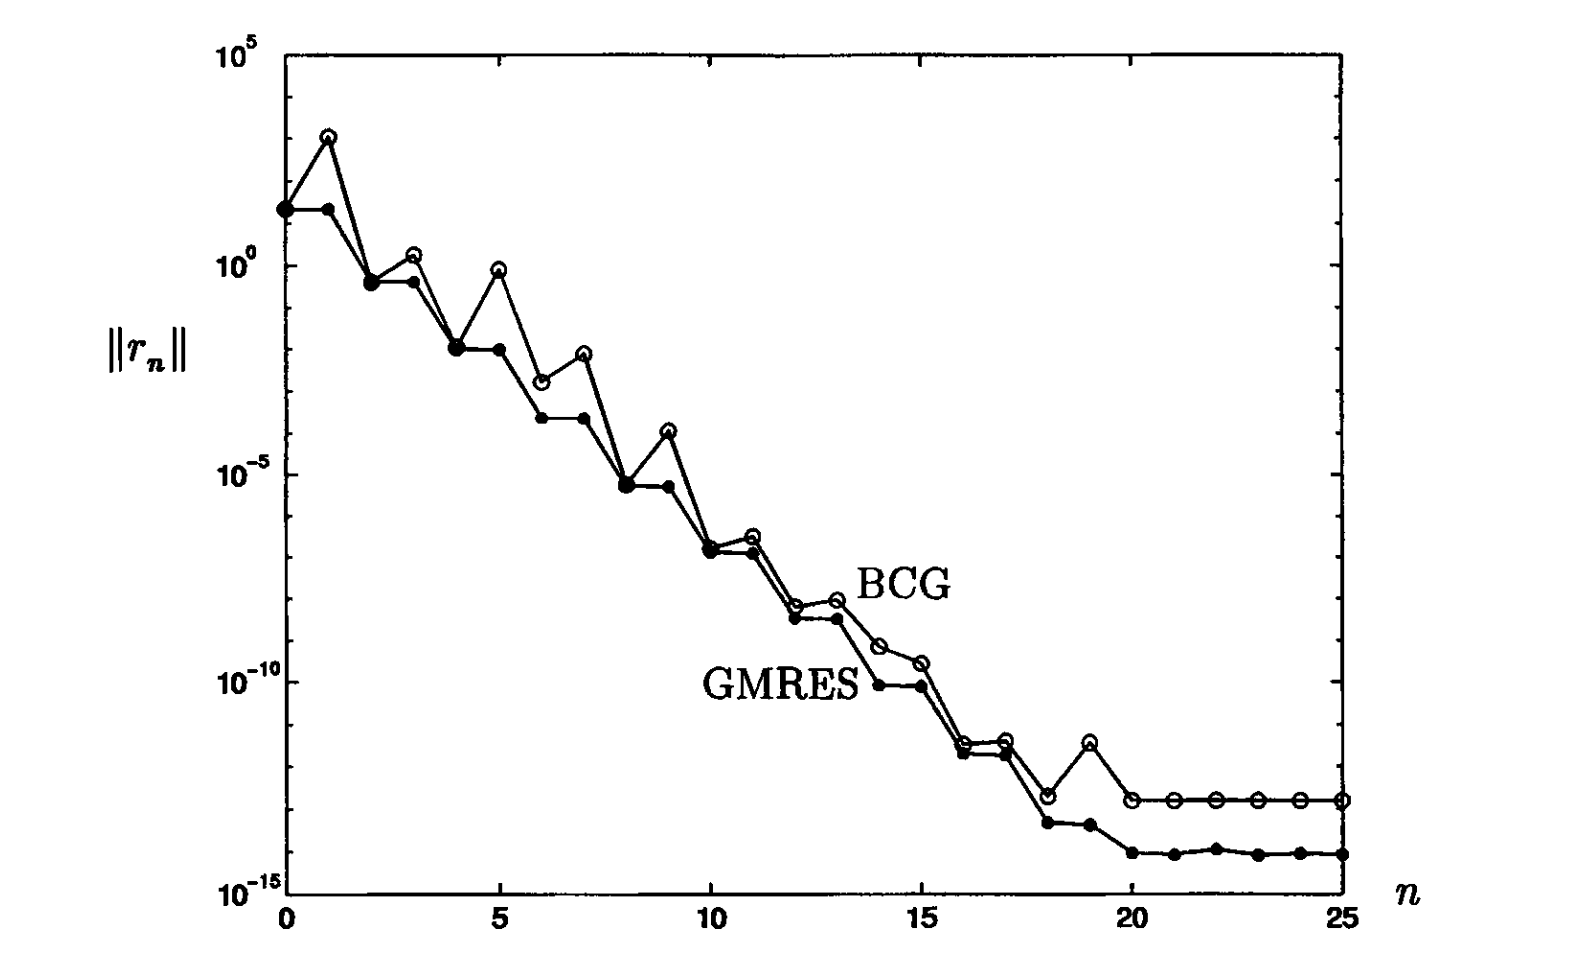
\includegraphics[width=0.8\textwidth]{figures/39-2.png}
    \caption{Comparison of GMRES and BCG for the $500 \times 500$ matrix labeled $\tau=0.01$ in Figure 38.1 , but with the signs of the entries randomized.}
\end{figure}
%────────────────────────────────────────

The horizontal axis in Figure 39.2 is the step number $n$, which is not the same as the computational cost. At each step, GMRES requires one matrixvector multiplication involving $A$, whereas BCG requires multiplications involving both $A$ and $A^*$. For problems where matrix-vector multiplications dominate the work and enough storage is available, GMRES may consequently be twice as fast as BCG or faster. 


\section{QMR and Other Variants} 
 
BCG has one great advantage over GMRES: it involves three-term recurrences, enabling the work per step and the storage requirements to remain under control even when many steps are needed. On the other hand, it has two disadvantages.
\begin{itemize}
    \item One is that in comparison to the monotonic and often rapid convergence of GMRES as a function of step number, its convergence is slower and often erratic, sometimes far more erratic than in Figure 39.2. Irregular convergence is unattractive, and it may have the consequence of reducing the ultimately attainable accuracy because of rounding errors. 
    \item The other problem with BCG is that it requires multiplication by $A^*$ as well as $A$. Depending on how these products are implemented both mathematically and in terms of computer architecture, this may be anything from a minor additional burden to effectively impossible.
\end{itemize}

In response to these two problems, beginning in the $1980 \mathrm{~s}$, more than a dozen variants of BCG have been proposed. Here are some of the best known of these; references are given in the Notes.
\begin{itemize}
    \item Look-ahead Lanczos (Parlett, Taylor, and Liu, 1985)
    \item $C G S=$ conjugate gradients squared (Sonneveld, 1989)
    \item $Q M R=$ quasi-minimal residuals (Freund and Nachtigal, 1991)
    \item $B i$-CGSTAB $=$ stabilized $B C G$ (van der Vorst, 1992)
    \item $T F Q M R=$ transpose - free $Q M R($ Freund, 1993)
\end{itemize}

The look-ahead Lanczos algorithm is based on the fact that when a breakdown is about to take place, it can be avoided by taking two or more steps of the iteration at once rather than a single step. The original idea of Parlett et al. has been developed extensively by later authors and is incorporated, for example, in the version of the QMR algorithm recommended by its authors. The phenomenon of breakdown can be shown to be equivalent to the phenomenon of square blocks of identical entries in the table of Padé approximants to a function, and the look-ahead idea amounts to a method of stepping across such blocks in one step. In practice, of course, one does not just test for exact breakdowns; a notion of near-breakdown defined by appropriate tolerances is involved.

The CGS algorithm is based on the discovery that if two steps of the BCG are combined into one in a different manner, so that the algorithm is "squared," then multiplication by $A^*$ can be avoided. The result is a "transpose-free" method that sometimes converges up to twice as quickly as BCG, though the convergence is also twice as erratic.

The QMR algorithm is based on the observation that although three-term recurrences cannot be used to minimize $\left\|r_n\right\|$, they can be used to minimize a different, data-dependent norm that in practice is usually not so far from $\left\|r_n\right\|$. This may have a pronounced effect on the smoothness of convergence, significantly reducing the impact of rounding errors. The Bi-CGSTAB algorithm is another method that also significantly smooths the convergence rate of BCG, and TFQMR is a variant of QMR that combines its smooth convergence with the avoidance of the need for $A^*$.

Most recently, efforts have been directed at combining these three virtues of smoothed convergence curves, look-ahead to avoid breakdowns, and transposefree operation. So far, all three have not yet been combined fully satisfactorily in a single algorithm, but this research area is young.